\documentclass[10pt]{article}
\usepackage[a4paper, total={170mm, 257mm}]{geometry}

\usepackage[
backend=biber,
style=nature,
sorting=none
]{biblatex}
\addbibresource{References.bib}
%\bibliographystyle{unsrt}


\usepackage{amsmath}
\usepackage{amssymb}
\usepackage{upgreek}
\usepackage{dsfont}
\usepackage{esint} % various fancy integral symbols
\usepackage{mathrsfs} % for \mathscr

% fancy notation stuff
\usepackage{accents}
% vector arrows under the symbol to distinguish covariant and contravariant
\newcommand\undervec[1]{\underaccent{\vec}{#1}}

\usepackage{siunitx}
\DeclareSIUnit{\litre}{l} % litres as lower case l (upper case L by default)

%\usepackage{hyperref}

\usepackage{graphicx} % Required for inserting images
\usepackage{multicol}
\usepackage{mathpazo}
\usepackage[font=sf,labelfont=bf]{caption}

% title, headings, abstract heading in sans serif font and maybe color
%\usepackage{sectsty}
%\usepackage{titling}
%\usepackage[sf,bf,pagestyles]{titlesec}
\usepackage[dvipsnames]{xcolor}
\usepackage{sectsty}
\usepackage{abstract}
\renewcommand\abstractnamefont{\sffamily\bfseries}%\color{Maroon}}
%\chapterfont{\color{blue}}  % sets colour of chapters
\sectionfont{\sffamily}%\color{Maroon}}  % sets colour of sections
\subsectionfont{\sffamily}%\color{Maroon}}  % sets colour of subsections
\subsubsectionfont{\sffamily}  % sets colour of subsections





% TO DO's
\newcommand{\todo}[1]{ {\color{ForestGreen} [#1]} }

\graphicspath{{figures/}}

\usepackage{lipsum} 

% referencing commands
\newcommand{\seefig}[2]{\mbox{\sffamily($\rightarrow$ Fig. \ref{#1}#2)}}
\newcommand{\reffig}[2]{\mbox{\sffamily{Figure \ref{#1}#2}}}


\title{\sffamily\bfseries\color{Maroon} Scattering Spectroscopy of\\Plasmonic Janus Particles}
\author{Felix H. Patzschke, A. Markus Anton and *Frank Cichos}
%\date{November 2023}
\date{}



\begin{document}
%\allsectionsfont{\sffamily}

\maketitle

\begin{abstract}\sffamily \vspace{-1em} 
%The light-matter interactions of plasmonic nanostructures are of great importance to [whom?].
%For plasmonic Janus particles in particular, which are established as an often-used tool in active matter research, the [???] is two-fold. [...]
%Metal-coated Janus particles have established themselves as a valuable tool in active matter research \cite{MONA-flow-fields} and related fields, owing to their plasmonically active nanostructures which allow for both excellent visibility in dark-field applications, as well as for efficient heating and, consequently, motility. \cite{MONA-thermotaxis, MONA-photon-nudging-1} 
%With light-matter interactions enhanced through their plasmonically active nanostructures, metal-coated Janus particles allow for both excellent visibility in dark-field applications as well as efficient heating and, consequently, motility \cite{MONA-thermotaxis, MONA-photon-nudging-1}, making them a valuable tool for active matter research. \cite{MONA-flow-fields}
%In recent years, theoretical predictions have been made of counter-intuitive optically enabled behaviours of such particles. \cite{Ilic2017}
%Nonetheless, these light-matter interactions are not yet thoroughly understood; in particular, there does not yet exist a proven method of inferring the out-of-image-plane orientation of a spherical Janus particle from its dark-field image. 
%Nonetheless, these light-matter interactions are not yet thoroughly understood.

%We present an experimental method for the orientation-dependent scattering spectroscopy of such anisotropic microscale particles. 
% $\SI{1}{\micro\meter}$ PS + $\SI{50}{\nano\meter}$ Au
%We analysed the scattering behaviour of \mbox{1µm PS + 50 nm Au} Janus Particles, resolving for wavelength, direction of illumination and scattering angle.
%under dark-field illumination and reproduced the results by finite-elements simulations. 
%We find well-discernible spectral features, particularly in the NIR range, that appear or disappear, depending on the orientation of the JP. 
%Further, we reproduced the experimental results by finite-element simulations.
%These findings may be worked into a method of determining the notoriously elusive out-of-plane orientation of spherical JPs, possibly even in real-time.

%We identify spectral markers, particularly in the near infrared range, that depend heavily on the orientation of the Janus particle; a result that may enable a new method of determining the notoriously elusive [to do: reference] out-of-plane orientation of spherical JPs, possibly even in real-time.
Plasmonic Janus particles consist of dielectric core particles with a thin metallic cap on one side and are widely used in active matter research. \cite{MONA-flow-fields} 
The plasmonic cap enhances optical scattering and absorption, allowing for self-propulsion through temperature gradients as well as efficient trapping and tracking. \cite{MONA-thermotaxis, MONA-photon-nudging-1} 
The asymmetry of such a particle gives rise to surface plasmon modes whose excitation is sensitive to the angle at which the particle is illuminated. 
Even though the angle of illumination strongly influences the particle's scattering response, the optical properties of such metallic caps have hardly been investigated. 

We probe the light scattering of individual micrometre-sized, spherical, Au-coated Janus particles by means of Selective Illumination Multiplexed Fourier Plane Spectroscopy. 
This novel method allows us to explore microparticles' scattering characteristics resolved for wavelength, angle of illumination and scattering angle. 

In addition, we supplement our experimental results with finite-element simulations and correlate spectral markers to orientation-dependent surface plasmon modes. 
This additional information on the correlation of angular and spectral information could pave the way for new methods of orientation detection. They also shed new light on the interaction of such spherically capped particles with light inducing forces and torques. \cite{Ilic2017, BA}
 \\ \end{abstract}





\begin{multicols}{2}

\section*{Introduction}

%\lipsum[1-3]

Janus particles (JPs) with a plasmonically active cap are a widely-used tool in active matter research: 
Through the absorption of visible light, the cap can be heated efficiently. 
In conjunction with the anisotropy of the particle, this facilitates directed self-propulsion. 
Meanwhile, the enhanced optical scattering of the cap leads to good visibility in microscopy, particularly in the dark field, which, in turn, allows for accurate tracking of the motile particles. 

As widely applicable as these particles' light-matter interactions (LMIs) may be, the are certainly not trivial: 
The length scales of the surface curvature are in the same order of magnitude as the wavelengths of light in the interaction, such that approximations along the lines of ray optics or dipole scattering are invalid. 
In addition, the asymmetry of the particles leads to orientation-dependency of the LMI. 
These orientation-dependencies may manifest in counter-intuitive ways: 
Some purely numerical studies suggest that plasmonic JPs can stably rotate, powered by a linearly polarized light field. \cite{Ilic2017,BA}

To our knowledge, this manner of LMIs has not yet been systematically studied. 
Orientation-dependent scattering studies of plasmonic nanostructures\footnote{specifically, Au nano-rods and -triangles, sized between 100 and 150 nm} \emph{have} been performed, \cite{Islam2021} but neither on JPs nor with a capacity for spectral resolution beyond RGB-decomposition. 
Moreover, no regard was given to the angular distribution of the scattered light.\footnote{which on such small objects isn't necessary - the angular distribuions look pretty much the same - but for larger particles, the differences in the shapes of the Mie plots can lead to drastic differences between the "true" scattering spectra and the measured ones.} 

We present an experimental method, which we use to study the LMI of plasmonic JPs consisting of a spherical polystyrene (PS) particle, $\SI{1}{\micro\meter}$ in diameter, with a $\SI{50}{\nano\meter}$ thick gold layer as the cap. 
We resolve the intensity of scattered light for wavelength and scattering angle. 
Though the theory of Mie \cite{Mie1908} only makes predictions for maximally symmetric particles, it serves well as reference in the characterization of the LMI of plasmonic JPs. 
We complement the measurement results with numerical simulations and find a good match between both methods' results. 
Through the analysis of the simulation results, we correlate peaks in the scattering spectra to orientation-dependent surface plasmon modes. 




\begin{figure*}[t]
    \centering
    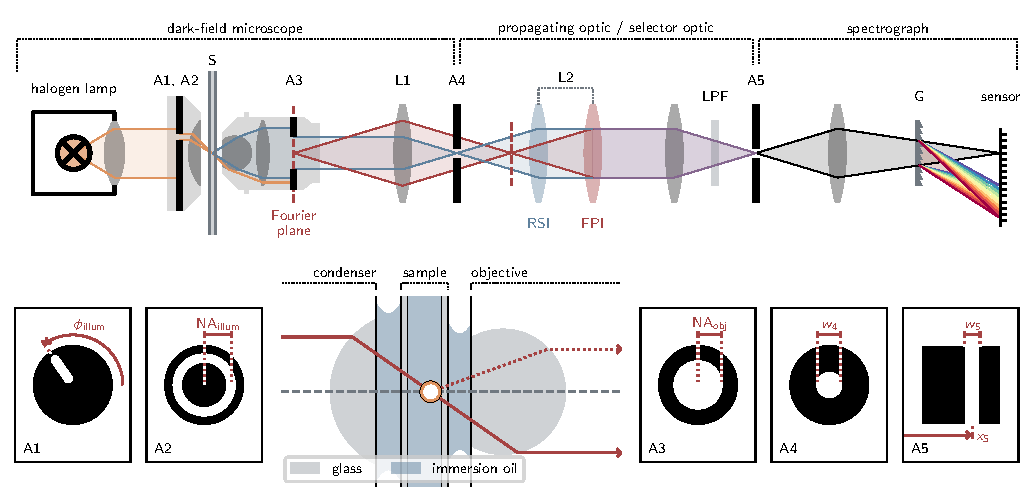
\includegraphics[width=\textwidth]{[fig] setup}
    %\includegraphics[width=\textwidth]{(fig) optics}
    \caption{
    Schematics of the imaging optics: 
    {\sffamily\bfseries (top)} The dark-field condenser directs the illumination (yellow light path) onto the sample {\sffamily (S)}; the apertures {\sffamily A1} and {\sffamily A2} restrict the direction of illumination. 
    In the immediate surroundings of the particle under observation {\sffamily\bfseries (bottom center)}, the ambient refractive index is virtually homogenous, due to the usage of immersion oil inside the sample.  
    The illuminating light is intercepted by the objective's aperture {\sffamily (A3)}, while scattered light from objects in the sample is allowed through. 
    The lens {\sffamily L1} produces an image of the sample in the plane of the aperture {\sffamily A4} and an image of the back aperture of the objective (Fourier plane) behind {\sffamily A4}, in the plane marked by the red dashed line. 
    The lens {\sffamily L2} can be moved between the real-space imaging ({\sffamily RSI}, blue) and the Fourier plane imaging ({\sffamily FPI}, red) position, each propagating an image of the corresponding plane onto the slit {\sffamily A5}, which functions as the entrance aperture of the spectrograph. 
    Inside the spectrograph, the image from {\sffamily A5} is propagated onto the camera sensor. 
    A diffraction grating produces a spectrally dispersed image, from which spectral data can be read. 
    An optional optical long-pass filter {\sffamily LPF} can be used to remove overlap between the first- and second-order 
    %{\sffamily\bfseries A1-A5:} Schematics of all apertures in the optical path. 
    }
    \label{fig:setup}
\end{figure*}

\section*{Simulations}
Numerically, the properties of the scattered light field were obtained using COMSOL Multiphysics. 
\todo{Intro to the geometric model. The COMSOL model is qualitatively the same as in \cite{BA}. } 
The surrounding medium was modelled with a refractive index of $1.51$. 

Given a plane wave 
$$
    \vec{E}_\mathrm{incident}(\vec{x},t) = \vec{E}_0 \cdot \exp\!\left( \mathfrak{i}\ \vec{k}\cdot\vec{x} - \mathfrak{i}\ \omega\ t \right)
$$
as the incident field, the solver produced a point-wise solution 
$$
    \vec{E}(\vec{x},t) = \vec{E}_\mathrm{incident}(\vec{x},t) + \vec{E}_\mathrm{sca}(\vec{x},t)
$$ 
to Maxwell's field equations on the defined geometry, where $\vec{E}_\mathrm{sca}(\vec{x},t)$ is the scattered field. 

The scattering cross-section of the particle was calculated from the scattered field as 
$$
    \sigma_\mathrm{sca} = \frac{2 \mu_0 \mu_r}{ {\bigl\Vert \vec{E}_0 \bigr\Vert}^2 } \cdot \oint_{\partial V} {\left\langle \vec{S}_\mathrm{sca} \right\rangle}_t \cdot\mathrm{d}\vec{A} \ ,
$$
where $\vec{S}_\mathrm{sca}$ is the Poynting vector of the scattered field and $\langle\cdot\rangle_t$ denotes the time average. 

\todo{Explanation on how the scattering intensity is resolved for $\hat{k}$} 
The scattered field can, according to Fourier's theorem, be decomposed into plane-wave components
$$
    \mathrm{d}\vec{E}(\vec{x},t) := \vec{\mathcal{E}}(\vec{k}) 
    \cdot 
    \exp{\!\left(\mathfrak{i}\ \vec{k}\cdot\vec{x} - \mathfrak{i}\ \omega\ t \right)}
    \ \mathrm{d}^3 k
    \ , 
$$
such that $ \vec{E}_\mathrm{sca} = \iiint_{\mathds{R}^3}\ \mathrm{d}\vec{E}$. 
The amplitudes $\vec{\vec{\mathcal{E}}}(\vec{k})$ of the components are given by the Fourier transform of $\vec{E}(\vec{x},t)$. 
The intensities of the components are given by 
$$
    \mathrm{d}\mathcal{I}(\vec{k}) = \frac{ \left\langle {\left\Vert \vec{\mathcal{E}}(\vec{k}) \right\Vert}^2 \right\rangle_t }{ 2\mu_0 \mu_r } \ \mathrm{d}^3k
    \ .
$$

With any fixed wavelength $\lambda$, the wavevectors are conveniently expressed as $ \vec{k} = 2 \pi \lambda^{-1} \cdot \hat{k} $, where \mbox{$\hat{k} \in \mathcal{S}^2$} is a unit vector. 
One obtains the spectral and angular distribution of scattered light, $\mathrm{d}\mathcal{I}(\lambda, \Omega)$, where $\Omega$ parametrizes the 2-sphere. 



\section*{Simulation Results}

\todo{A summary figure of sim results: scattering spectra, Mie plots and the like}

\todo{We find that the scattering cross-section heavily depends on the orientation of the JP.}

Over the spectral range that we analyzed, though decidedly not in general, the scattering efficiency of the particle was ... greater if it was illuminated from either the Au or the PS side than if it was illuminated side-on. 
In both cases, the scattering spectra have multiple peaks. 
Between axial and side-on illumination, though, there is no clear correspondence between these peaks. 

E.g., for side-on illumination, there is a scattering peak at $\lambda\approx\SI{540}{\nano\meter}$, that has no counterpart in the spectra for axial illumination. 
We ascribe this peak to the nanostructure plasmon resonance of gold: 
It sits right around that wavelength and it is only under side-on illumination that the incident electric field may be perpendicular to the surface of the Au cap at its points of highest curvature, that being the cap's perimeter. 

The more immediately noticeable feature of the scattering spectra is the pair of peaks at $\lambda\approx\SI{1000}{\nano\meter}$,\footnote{precisely, they are at 996.9 nm and 998.9 nm, respectively.} which only appears under axial illumination. 
As $\hat{k}$ is parallel to the symmetry axis of the JP, the perimeter of the Au cap is coplanar to the electric field and a resonant surface plasmon is excited in it. 

Neither of these peaks is present\footnote{discernable?} in the scattering spectrum of an equivalently sized Au sphere. 




\section*{Experiments}

\subsection*{Sample Preparation}

The JPs were produced by \todo{cite production from Nic's work} and consist of spherical PS beads, coated with a layer of gold, $\SI{50}{\nano\meter}$ thick on average, on one side, with a $\SI{5}{\nano\meter}$ thick layer of chromium as a binding agent in between. 
A $\SI{30}{\micro\litre}$ droplet was placed on a cover slip and the JPs in solution were left to sediment for \mbox{10 minutes}. 
Afterwards, the solvent was blown off using nitrogen gas, leaving the remaining JPs stuck on the coverslide. 
A second cover slip was placed on top, with a droplet of $\SI{1.5}{\micro\litre}$ of immersion oil\footnote{TO DO: serial number} in between, such as to keep the ambient refractive index constant in the vicinity of the particles.   

\subsection*{Setup}

The imaging setup is sketched in \reffig{fig:setup}{C}. 
Its basis was formed by a standard dark-field microscope. 
A confocal aperture in the image plane of the dark-field microscope was used to isolate the scattered light from a single JP. 
At the other end of the optical path stood a homebuilt spectrograph, consisting of 
\begin{itemize}
    \item an sCMOS camera \mbox{\sffamily(pco.edge 4.2)} for image acquisition, 
    \item a transmissive diffraction grating {\sffamily(ThorLabs GTI25-03A)} in front of it, used for spectral dispersal of the image,
    \item a tunable slit to select only a thin vertical line from an image in order to prevent overlap of spectrally dispersed signals from different points in the original image and
    \item a lens to propagate the image from the plane of the slit onto the camera sensor.  
\end{itemize}

Both sub-assemblies were linked by a propagating optic, with which either the image plane wherein the aperture lay or the back focal plane (BFP) of the microscope objective could be chosen to be projected onto the slit.

\begin{figure*}[t!]
    \centering
    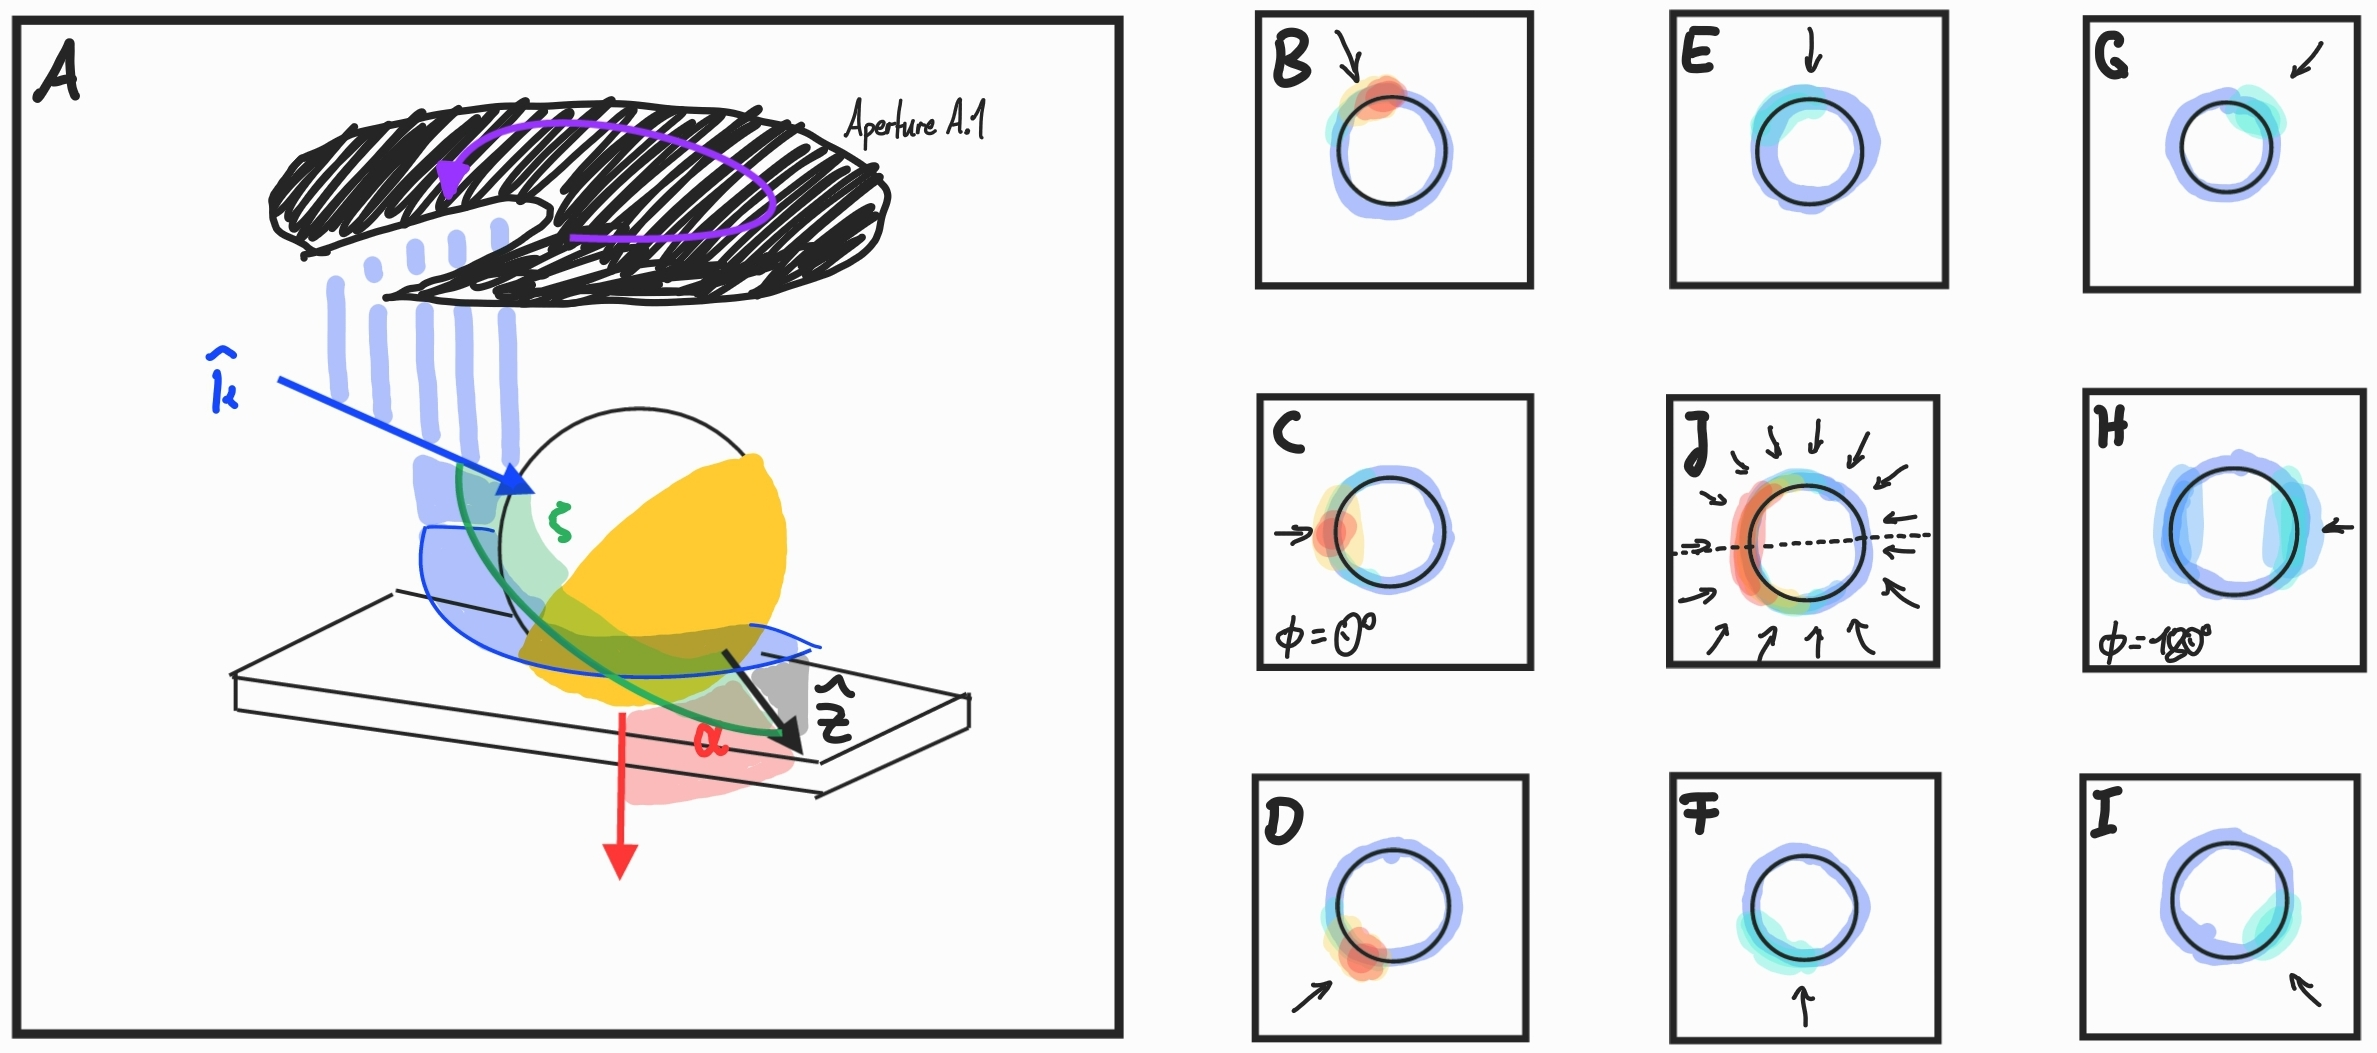
\includegraphics[width=\textwidth]{[fig] selective illumination}
    \caption{Selective Illumination:   
    {\sffamily\bfseries A:} By rotating the aperture A.1 the direction of illumination on the particle can be controlled within the range permitted by its out-of-plane orientation. 
    {\sffamily\bfseries B-I:} Dark-field images of a JP under restricted illumination. 
    The arrows signify the in-plane angle of the illumination.  
    {\sffamily\bfseries J:} The same JP under unrestricted (normal) dark-field illumination. 
    }
    \label{fig:selective-illumination}
\end{figure*}

The real-space-imaging mode was used to select particles for measurement as well as for spectral measurements in which the scattering angle was not resolved. 
The BFP-imaging mode was used to align the dark-field illumination and to record spectrally resolved Fourier-space images of the JP under observation. 
To that end, the front aperture of the spectrograph (i.e. the slit) was slowly translated across the BFP image while recording, such that the camera would record one spectrally dispersed vertical line of the BFP image at a time. 
The accumulation time for one such dataset was approximately \mbox{15 minutes}.  

The calibration data for the wavelength-dependent sensitivity of the optics was collected by allowing the illumination light to pass through the entire assembly and recording its spectrum. 

For the samples, a drop of the JP solution was placed on a cover slip and the particles were allowed to sediment for at least \mbox{5 minutes}. 
Then, the solvent was blown off the cover slip with compressed air. 
A second cover slip was placed atop the first one, with a drop \mbox{$(\sim 1.5\,\mathrm{\upmu l})$} of immersion oil in between, ensuring no significant changes in the ambient refractive index in the vicinity of the JPs. 

\subsection*{Global Illumination}

[...]

For validation, the scattering spectra of $\SI{65}{\nano\meter}$ AuNPs were measured. 
Such small particles were chosen for two reasons: 
a) The resonance in the expected scattering spectrum would be as narrow as possible and b) the shape of the angular distribution of scattered light would not change appreciably over the spectral range of interest, causing the measured and full scattering cross-sections to only differ by a constant factor. 
In the comparison of the measured spectra to the predictions of Mie theory \cite{Mie1908, BohrenHuffman, GouesbetGrehan} using the values by Johnson \& Christy \cite{Johnson1972} for the complex refractive index of gold shows a strong agreement. 

\begin{figure*}[t]
    \centering
    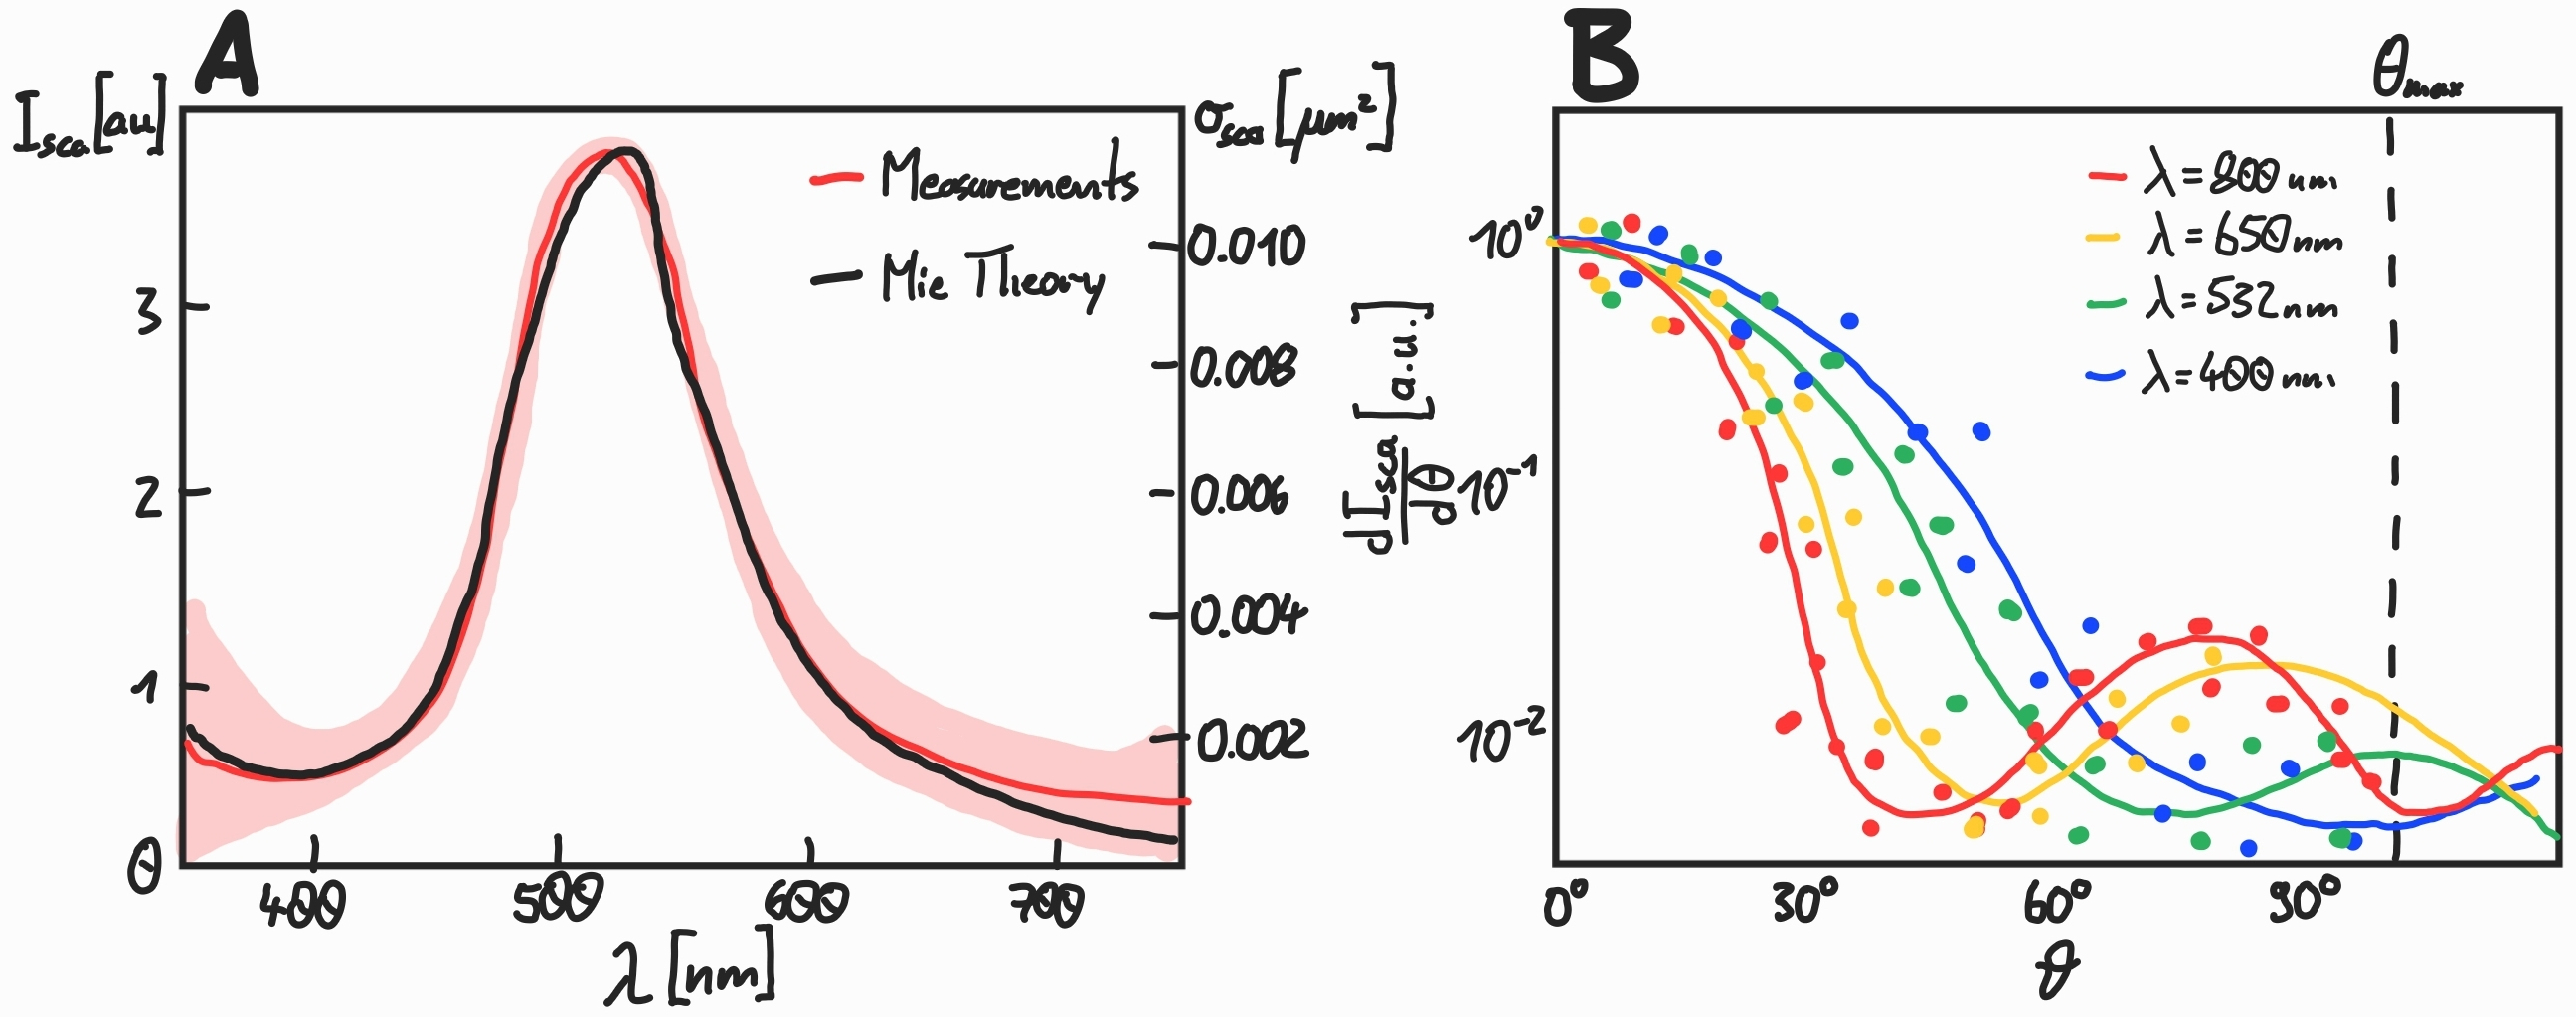
\includegraphics[width=\textwidth]{[fig] AuNP (placeholder).jpg}
    \caption{(Placeholder) 
    {\sffamily\bfseries A:} Scattering spectrum of 65 nm Au NPs. The shaded area corresponds to the SNR. 
    {\sffamily\bfseries B:} Scattering intensity of a spherical Au NP, $d=\SI{250}{\nano\meter}$ versus the scattering angle for various wavelengths. The lines show the predictions of GLMT \cite{GouesbetGrehan}, the points show measurement results.
    }
    \label{fig:AuNP}
\end{figure*}

Recorded scattering spectra of the JPs are shown in \reffig{fig:spectra}{B}.

\subsection*{Orientation Dependent}

\begin{figure*}[t!]
    \centering
    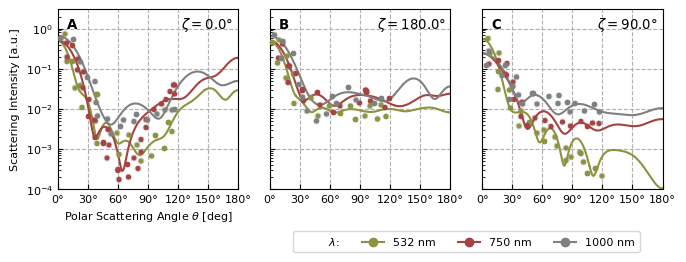
\includegraphics[width=\textwidth]{[fig] cartesian mieplots (3, placeholder)}
    \caption{Scattering intensity of the JP versus scattering angle. 
    The points signify measured intensities while the lines are simulation results.  
    {\sffamily\bfseries A} and {\sffamily\bfseries B} show the cylindrically symmetric cases of illumination from the PS side and from the Au side, respectively, i.e. where $\hat{k}\parallel\hat{z}$. 
    In {\sffamily\bfseries C}, the light is incident side-on ($\hat{k}\perp\hat{z}$, $\zeta=\pi/2$). 
    Disregarding the local extrema, qualitatively distinct large-scale behaviour is apparent: Under illumination from the PS side {\sffamily\bfseries (A)}, the scattering intensity becomes globally minimal in the sideways direction. 
    Meanwhile, under illumination from the Au side {\sffamily\bfseries (B)}, it reaches a plateau and under side-on illumination {\sffamily\bfseries (C)}, the scattering intensity drops consistently between forwards and backwards.  
    }
    \label{fig:jp-mieplots-oneline}
\end{figure*}

\section*{Simulation \& Emulation}

The finite-element simulations were performed in COMSOL \mbox{Multiphysics 6.1}. 
%The simulation per se is ignorant of real-world optical devices and.
%Therefore, the geometric definition of the model does not depend on \mbox{$\hat{o}$-direction} or the objective aperture. 
The model geometry was defined in particle-coordinates, i.e. $\hat{z}$ coincides with the $z$-axis. \cite{BA} 

Essentially, the solver is provided with an analytic expression for the incident electric field
$\vec{E}_\mathrm{inc}(\vec{x},t)$
and returns samples for the scattered field
$\vec{E}_\mathrm{sca}(\vec{x},t)$, 
such that the total electric field 
$$\vec{E}(\vec{x},t) = \vec{E}_\mathrm{inc}(\vec{x},t) + \vec{E}_\mathrm{sca}(\vec{x},t) $$
satisfies Maxwell's field equations. 

For the incident field, a plane wave was given, wherein the illumination angle $\zeta$ is encoded as a rotation of the incident light field in the $(x,z)$ plane: 
$$
    \vec{E}_\mathrm{inc} = \vec{E}_0 \cdot \mathrm{exp}\left( \mathfrak{i} \, \vec{k} \cdot \vec{x} - \mathfrak{i} \, \omega \, t \right)
$$
with $\omega = 2\pi\,c/\lambda$, as well as
$$
    \vec{E}_0 = E_0 \cdot \boldsymbol{R}_{\hat{k}}^{\chi} \cdot \boldsymbol{R}_{\hat{y}}^{\zeta-\frac{\pi}{2}} \cdot \hat{z}
    \quad\text{and}\quad
    \vec{k} = \frac{2\pi}{\lambda} \cdot \overbrace{ \boldsymbol{R}_{\hat{y}}^{\zeta} \cdot \hat{z} }^{\hat{k}}
    \ ,
$$
where $\chi$ is the polarisation angle of the incident light field. % and $\boldsymbol{R}_{\hat{a}}^{\alpha}$ denotes the right-handed rotation around the angle $\phi$ and the axis defined by the unit vector $\hat{a}$. 

The intensity of the incident field is 
$$I_0 = \frac{1}{2\mu_0 \mu_r} {E_0}^2 \ .$$
\cite{Griffiths-ED,MA}



\subsection*{Measurement Emulation}

To emulate the unpolarised light that the measurements were conducted with, $\chi$ was sampled as \mbox{$\in\left\lbrace0, \pi/2\right\rbrace$} and, in the evaluation, intensities were averaged.\footnote{This is allowed because $I\propto\left\Vert \hat{E} \right\Vert^2$.}

Through a Fourier transform, the scattered field is decomposed into plane-wave components:
$$
    \vec{E}_\mathrm{sca}(\vec{x},t) = \iiint_{\mathds{R}^3} \vec{\mathfrak{E}}(\vec{k}) \cdot \exp\!\left( \mathfrak{i}\,\vec{k}\cdot\vec{x} - \mathfrak{i}\,\omega\,t\right) \mathrm{d}^3 \vec{k} \ .
$$


The measured scattering cross-section of the JP corresponds to the sum of the intensities of all plane-wave components of the scattered field that enter the measurement optics:
$$\sigma_\mathrm{sca,measured} \propto \iint_{\mathcal{D}} I\left( \hat{k}' \right) ~\mathrm{d}\Omega\ ,$$
Where $\mathcal{D} \subseteq \mathcal{S}^2$ is the set of propagation directions $\hat{k}'$, for which a plane wave component will contribute to the signal on the detector. 
In the experiment, the requirement is for it to enter the objective, and thus
$$
    \mathcal{D} = \left\lbrace\ \hat{k}' \in \mathcal{S}^2\ \middle\vert\ \measuredangle\!\left( \hat{k}', \hat{o}\right) < \theta_\mathrm{NA}\ \right\rbrace
    \ ,
$$
where $\theta_\mathrm{NA}$ is the opening angle of the objective's collection cone, given by the numerical aperture,
$$\theta_\mathrm{NA} = \mathrm{asin}\frac{\mathrm{NA}}{n} \ .$$

\begin{itemize}
    \item The simulation provides values of the scattered field for sampled values of $\zeta$.
    \item The numerical aperture of the dark-field condenser defines $\measuredangle(\hat{k},\hat{o})$.
    \item The out-of-plane angle $\alpha$ of the JP is unknown and not uniquely defined by $\zeta$ and $\measuredangle(\hat{k},\hat{o})$. We sample $\alpha\in\left[0,\pi\right]$ and weight the results by $p(\alpha) = \sin\alpha$.\footnote{$p(\alpha)$ is the probability density function for the out-of-plane angle of a randomly oriented spherical JP. For the derivation, see the supplementary material.}
\end{itemize}


Both the experiment and the simulations show that, in asymmetric cases, light is preferentially scattered in the direction of the Au cap.





\begin{figure*}[t]
    \centering
    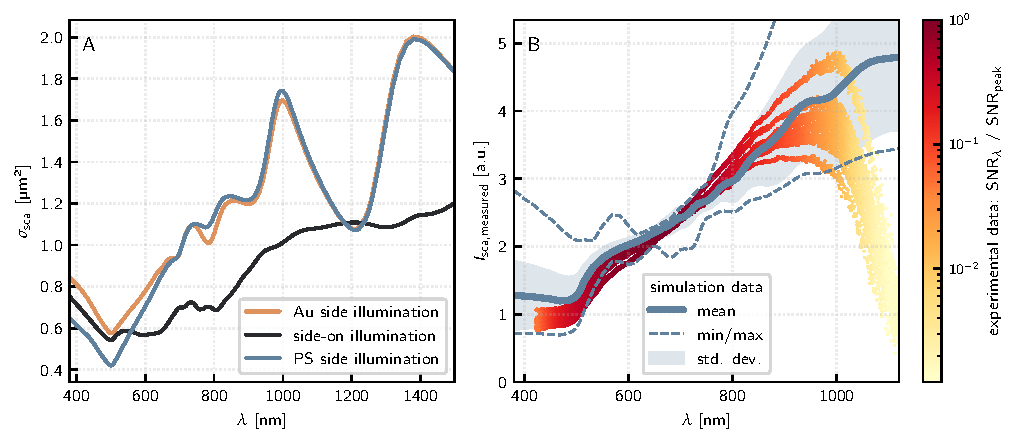
\includegraphics{[fig] spectra.PDF}
    \caption{{\sffamily\bfseries A:} simulated scattering spectrum of the JP under illumination from the Au side (yellow), from the PS side (blue) and from the equatorial side (black). {\sffamily\bfseries B:} measured scattering spectra (orange) atop value range as determined by simulation + emulation (blue).}
    \label{fig:spectra}
\end{figure*}

\section*{Discussion}

Notable findings are...
\begin{itemize}
    \item The spectral bump at $\lambda\approx\SI{550}{\nano\meter}$. It's discernable in both real and emulated measurements, though in the raw simulation data it only appears for side-on illumination. 
    It's likely the same peak as would show up for an arbitrarily small Au NP. 
    The plasmon mode is excited in the rim of the cap by electric fields that are perpendicular to the Au surface at its point(s) of highest curvature. (i.e. $\vec{E} \parallel \hat{z}$, which can only happen if $\hat{k} \perp \hat{z}$)
    \item The clearly discernable peak at $\lambda\approx\SI{1000}{\nano\meter}$ is present under the opposite circumstances, i.e. when $\hat{k}\parallel\hat{z}$. 
    It corresponds to a surface plasmon resonance of the Au cap. (Polar/Azimuthal?\footnote{Rim modes can, when $\hat{k}\parallel\hat{z}$, only really be excited in the fundamental mode. The same should go for azimuthal modes. right?})
    \item Comparing the angular distributions to those of a Mie particle, there is clear similarity: 
    Non-global maxima become more well-distinguished and over-all fewer as wavelength increases. 
    The same happens as the direction of illumination is changed from $\hat{k}\perp\hat{z}$ to $\hat{k}\parallel\hat{z}$: Both transitions can, from a Mie-theoretical point of view, be understood as a decreasing size parameter. (consider the ratio of the effective diameter\footnote{"depth"?} of the plasmonic structure in the direction of the wave propagation to the wavelength)  
    \item The out-of-plane orientation of the JP is not easy to infer: 
\end{itemize}

It is notable that the bump at \mbox{$\lambda \approx \SI{550}{\nano\meter}$} that is discernible in both the real and the emulated measurements \seefig{fig:spectra}{A}, appears in the raw simulation data \seefig{fig:spectra}{B} only under side-on illumination, i.e. \mbox{$\zeta\approx\pi/2$}. 

\section*{Conclusion \& Outlook}

In summary, we conducted spectroscopic studies of the light scattering behaviour of individual, micrometre-sized Janus particles. 
We find that the anisotropy of the JP causes certain features to appear in and disappear from its scattering spectrum under certain orientations, particularly in the NIR range. 

An experimental setup that can detect these features, possibly even in real time, is feasible.

Interesting things to do with this in the future might be...
\begin{itemize}
    \item Direct analysis of the surface plasmons: 
    Decomposition of the tangential electric field in an appropriate basis (vector hemispherical harmonics?) to find relative excitation of every (important) surface plasmon mode, depending on wavelength and illumination angle.
    \item Real-time spectroscopy to track a JP's out-of-plane angle. 
\end{itemize}






%\section*{References}
\printbibliography

\section*{Acknowledgements}
[...]

\section*{Author Contributions}
%\textbf{F. C.} designed the experiment, [...] and reviewed the manuscript, \textbf{F. H. P.} designed the experiment, constructed the optical setup, performed the experiment, implemented the data analysis and wrote the manuscript.
F.C. and F.H.P. designed the experiments; 
F.H.P. constructed the optical setup, performed the experiments, implemented the simulations and conducted the data analysis; 
F.H.P. and A.M.A. and wrote the manuscript; 
All authors reviewed the manuscript.

\section*{Competing Interests}
The authors have no competing interests to declare. 

\section*{Additional Information}
[...]












\end{multicols}
















\end{document}
